\documentclass[pdftex,10pt,a4paper]{report}
\usepackage[usenames,dvipsnames]{color}
\usepackage{tikz}
\usepackage{graphicx}
\usepackage{setspace}
\usepackage{natbib}
\usepackage{url}
%% Define a new 'leo' style for the package that will use a smaller font.
\makeatletter
\def\url@leostyle{%
  \@ifundefined{selectfont}{\def\UrlFont{\sf}}{\def\UrlFont{\small\ttfamily}}}
\makeatother
%% Now actually use the newly defined style.
\urlstyle{leo}
\newcommand{\HRule}{\rule{\linewidth}{0.5mm}}
\begin{document}
%
\begin{titlepage}
\begin{center}
% Upper part of the page


\textsc{\color{Sepia}{\LARGE EC~320}}\\[1.5cm]
\textsc{\Large Week-Three}\\[0.5cm]
\textsc{\Large 3.5.3}\\[0.5cm]
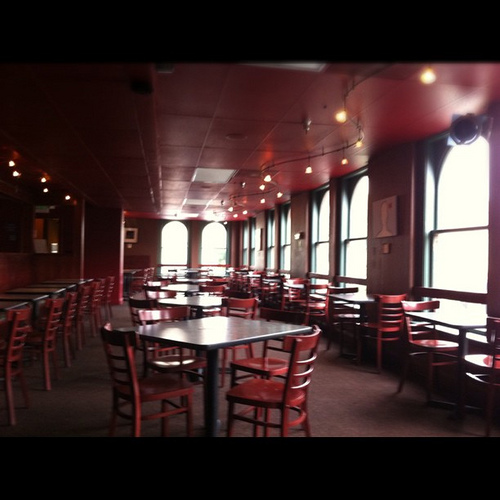
\includegraphics[scale=0.5]{GDP}\\
% Title
\HRule \\[0.4cm]
{ \huge \bfseries Startup America}\\[0.4cm]
\HRule \\[1.5cm]


% Author and supervisor
\begin{minipage}{0.4\textwidth}
\begin{flushleft} \large
\emph{Author:}\\
Jason \textsc{Mansfield}
\end{flushleft}
\end{minipage}
\begin{minipage}{0.4\textwidth}
\begin{flushright} \large
\emph{Instructor:} \\
Dr.~Anthony \textsc{Pizur}
\end{flushright}
\end{minipage}

\vfill

% Bottom of the page
{\large \today}

\end{center}
\end{titlepage}
\section{Entrepreneurs}
\begin{doublespace}
In  American society it seems easier to point fingers at others and mumble about how our economy is ruined. Granted it took alot of wall street greed to do so much damage to our economy as a whole. However, this is not the first time in American history where we have lived with a recession. Forbes.com authors remind us of our past~\cite{Linder:2011}: 
\end{doublespace} 
\begin{quote}
Take Charles Wiley, who opened a small print shop in lower Manhattan in 1807--the same year the U.S. Congress, provoked by a British warship that opened fire off the coast of Norfolk, Va., passed an embargo preventing American ships from landing at foreign ports unless authorized by President Thomas Jefferson himself.The economic warfare triggered a painful, seven-year recession, but Wiley soldiered on, partnering with Cornelius Van Winkle, a more established Manhattan printer. The two hosted a meeting place for famous scribes like James Fenimore Cooper and William Cullen Bryant and published future legends Edgar Allen Poe and Washington Irving. The company eventually expanded into textbooks and other higher-margin titles. Headquartered in Hoboken, N.J., John Wiley \& Sons now boasts a \$2 billion market capitalization on the New York Stock Exchange.
\end{quote}
\begin{doublespace}
While large business is failing to serve the common man through standard careers its time to create our own. Men and Women work for 10 to 30 years for large businesses which are corrupted and have little investment on the worker bees who keep them afloat.
\end{doublespace}
\clearpage
% bib stuff
    \nocite{*}
    \bibliographystyle{apalike}
    \bibliography{cite}

\end{document}


